% =============================================================================
%  Chapitre 5 — Résultats, validation et produit livré
%
%  Tous les chiffres cités proviennent des artefacts versionnés du projet
%  (data/gold/*.json) et sont repris à l'identique par les figures, produites
%  par scripts/build_figures_chap5.py. Aucun nombre n'est saisi manuellement,
%  de sorte que le rapport ne peut pas diverger des résultats qu'il décrit.
% =============================================================================

\chapter{Résultats, validation et produit livré}
\label{chap:resultats}

\section*{Comment lire ce chapitre}
\addcontentsline{toc}{section}{Comment lire ce chapitre}

Ce chapitre présente ce que le système produit réellement. Il est organisé selon
un principe simple, hérité du problème P4 exposé au
chapitre~\ref{chap:problematique} : \textbf{un chiffre n'est un résultat que si
l'on sait de combien il pourrait être faux.}

Chaque performance est donc rapportée avec son intervalle de confiance, et le
chapitre distingue explicitement trois catégories :

\begin{itemize}
  \item ce qu'il \textbf{observe} — des écarts historiques, sans les transformer
        en supériorité généralisable faute de test pairé ;
  \item ce qu'il \textbf{explore} — des associations sur un faible nombre
        d'événements, utiles pour orienter l'analyse mais non confirmatoires ;
  \item ce qu'il \textbf{réfute} — cinq pistes explorées et fermées.
\end{itemize}

Cette troisième catégorie n'est pas un aveu d'échec. Sur un sujet où la
littérature abonde en performances irreproductibles, une piste correctement
fermée a plus de valeur qu'une performance invérifiable.

% =============================================================================
\section{Le résultat principal}
% =============================================================================

Le système complet — détection de régime par chaîne de Markov cachée et
covariance dynamique — a été comparé aux trois approches classiques sur les deux
univers, hors échantillon et net de coûts de transaction.

\begin{table}[htbp]
  \centering
  \caption[Performance comparée, hors échantillon]{Performance nette de coûts,
  hors échantillon. \emph{DD} désigne le drawdown maximal (la pire perte
  pic-à-creux), et le ratio de Calmar rapporte le rendement à ce drawdown.}
  \label{tab:headline}
  \small
  \begin{tabular}{llrrrr}
    \toprule
    Univers & Stratégie & Sharpe & Rendement & DD max. & Calmar \\
    \midrule
    \multirow{4}{*}{\shortstack[l]{Portefeuille\\EURAFRIC\\(9 actifs)}}
      & \textbf{Système ML (régime)}      & \textbf{1,236} & 12,2~\% & $-14{,}1$~\% & 0,862 \\
      & Markowitz Sharpe max.             & 1,164 & \textbf{13,2~\%} & $-13{,}2$~\% & \textbf{1,000} \\
      & Équipondéré (1/N)                 & 1,160 & 11,6~\% & $-13{,}6$~\% & 0,852 \\
      & Variance min. (Ledoit-Wolf)       & 1,074 &  9,9~\% & $\mathbf{-12{,}8}$~\% & 0,775 \\
    \midrule
    \multirow{4}{*}{\shortstack[l]{ETF inter-\\nationaux\\(5 actifs)}}
      & \textbf{Variance min. (Ledoit-Wolf)} & \textbf{0,953} & 10,3~\% & $-26{,}9$~\% & 0,382 \\
      & Système ML (régime)               & 0,937 & 10,4~\% & $-26{,}9$~\% & \textbf{0,386} \\
      & Markowitz Sharpe max.             & 0,912 & \textbf{10,8~\%} & $-32{,}8$~\% & 0,329 \\
      & Équipondéré (1/N)                 & 0,769 &  9,6~\% & $-36{,}2$~\% & 0,266 \\
    \bottomrule
  \end{tabular}
\end{table}

Sur le portefeuille EURAFRIC, le système obtient un ratio de Sharpe de
\textbf{1,236} contre \textbf{1,164} pour la meilleure approche classique, soit
un gain de \textbf{$+6{,}2$~\%}. Sur l'univers ETF, il obtient 0,937 contre
0,953~: il \textbf{perd} de $1{,}6$~\%.

\begin{figure}[htbp]
  \centering
  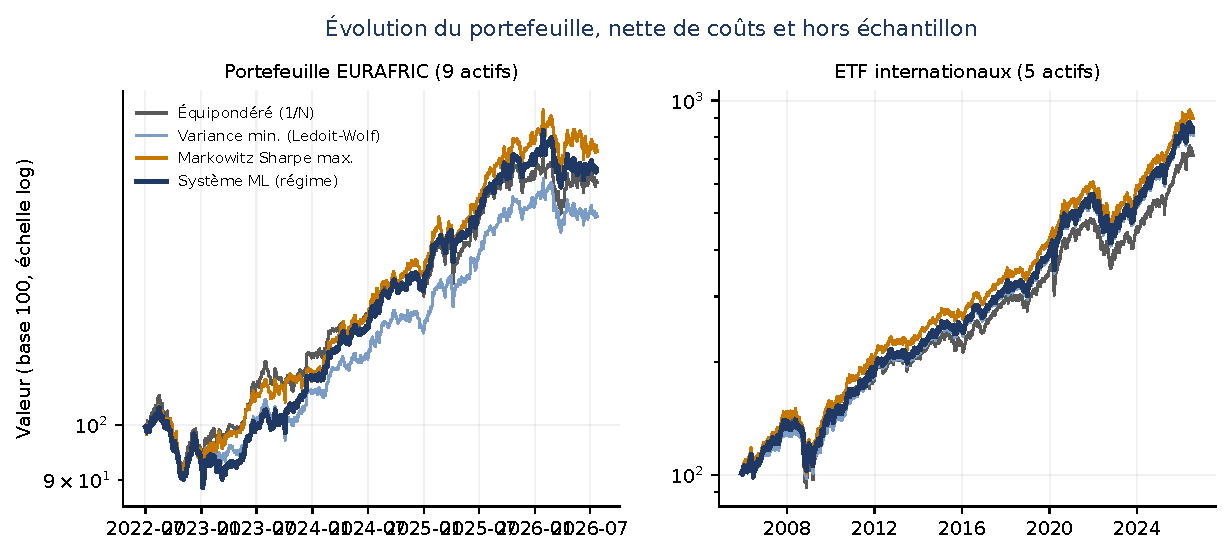
\includegraphics[width=\textwidth]{assets/figures/courbes_equity.pdf}
  \caption[Évolution des portefeuilles]{Évolution des portefeuilles, nette de
  coûts et hors échantillon (échelle logarithmique). Le système ML est tracé en
  trait épais. L'écart entre stratégies est faible au regard de l'amplitude des
  mouvements de marché — ce que la section suivante quantifie.}
  \label{fig:courbes}
\end{figure}

\begin{remarquebox}
Le résultat est donc \emph{mitigé, et il est rapporté comme tel}. Un système qui
n'apporterait un gain que sur l'univers où on a choisi de le mettre en avant ne
serait pas un système, mais une sélection.
\end{remarquebox}

\subsection{Une réserve sur le choix de la mesure}

Le tableau~\ref{tab:headline} appelle une observation que l'honnêteté impose de
formuler, car elle nuance le résultat principal.

Sur le portefeuille EURAFRIC, le système ML l'emporte \emph{au sens du ratio de
Sharpe} — mais il est battu par le Markowitz classique sur le rendement annualisé
(12,2~\% contre 13,2~\%), sur le drawdown maximal ($-14{,}1$~\% contre
$-13{,}2$~\%), sur le ratio de Calmar (0,862 contre 1,000) et sur le turnover
(0,29 contre 0,14, soit deux fois plus de transactions).

Autrement dit : \textbf{le gain provient d'une réduction de la volatilité, non
d'un supplément de rendement}, et il n'apparaît que dans la mesure qui divise par
cette volatilité. Un gérant dont le mandat privilégie le rendement par unité de
perte maximale — le critère de Calmar — préférerait le Markowitz classique.

Cette dépendance du classement au choix de la mesure est un résultat en soi. Elle
justifie que les sections suivantes ne s'appuient pas uniquement sur le ratio de
Sharpe.

% =============================================================================
\section{Ce chiffre est-il réel ? La validation hors échantillon}
% =============================================================================

Un écart de $+6{,}2$~\% mesuré sur une période unique ne dit rien tant qu'on
ignore sa marge d'erreur. Deux protocoles ont été appliqués pour l'établir.

\paragraph{Le test gelé.} Les derniers 35~\% de chaque univers ont été mis de
côté avant toute calibration. Les hyperparamètres des modèles ont été choisis sur
la partie restante par \textbf{validation strictement antérieure}
(\emph{forward-only}), puis \emph{figés} ; le verdict n'a été mesuré qu'une fois,
sur ce segment jamais vu.

Le mot « strictement » est le correctif apporté à ce protocole. La version
précédente employait une validation croisée purgée en blocs, qui entraîne le
modèle sur \emph{toutes} les dates hors de la bande de purge — y compris
\textbf{postérieures} au bloc de validation. C'est la construction canonique de
López de Prado, défendable lorsque les labels se chevauchent, mais elle note un
pli de 2018 avec un modèle ajusté en partie sur 2019--2024 : une question
qu'aucun gérant ne peut poser en direct. Chaque pli respecte désormais
\[
\text{fin\_entraînement} < \text{début\_embargo} \le \text{début\_validation}
\le \text{fin\_validation} < \text{début\_test}
\]
et la géométrie réellement appliquée — dates, effectifs, IC par pli — est publiée
dans \texttt{phase5\_\allowbreak validation\_\allowbreak protocol.json} plutôt qu'affirmée ici.

\paragraph{Le walk-forward imbriqué.} La fenêtre de test unique du protocole
précédent ne représente que 455~jours sur le portefeuille EURAFRIC, ce qui produit
des intervalles très larges. Un second protocole re-sélectionne la configuration à
six frontières successives et concatène chaque segment hors échantillon, portant
l'évaluation à \textbf{793~jours} — sans que la sélection ne voie jamais sa propre
fenêtre d'évaluation.

\begin{figure}[htbp]
  \centering
  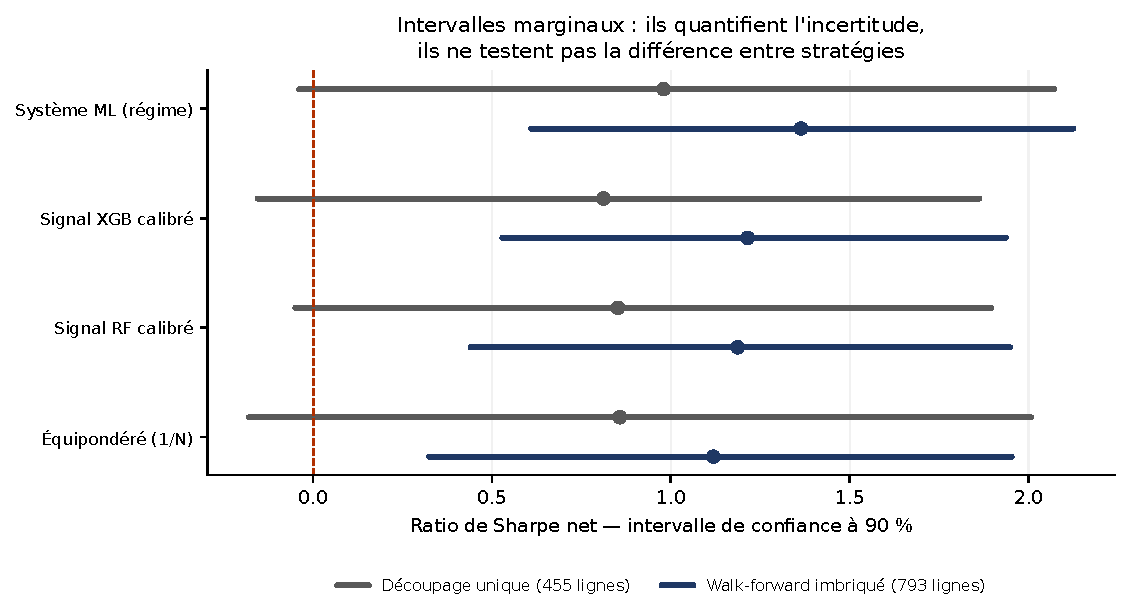
\includegraphics[width=\textwidth]{assets/figures/intervalles_confiance.pdf}
  \caption[Intervalles de confiance]{Ratios de Sharpe hors échantillon et
  intervalles de confiance à 90~\% (bootstrap par blocs), pour les deux
  protocoles. Le protocole imbriqué (bleu) resserre les intervalles de
  \textbf{28,6~\%} en moyenne. Les intervalles marginaux restent néanmoins
  largement chevauchants~: ils quantifient l'incertitude, sans constituer un
  test pairé de différence entre stratégies.}
  \label{fig:intervalles}
\end{figure}

\paragraph{Le test pairé — la preuve qui manquait.} Les intervalles ci-dessus
sont \emph{marginaux} : ils décrivent l'incertitude de \emph{chaque} stratégie
prise isolément. Ils ne testent pas si deux stratégies diffèrent, et les lire
ainsi est une erreur dans les deux sens — deux intervalles peuvent se chevaucher
largement alors que la différence pairée est systématiquement positive (les
stratégies partagent les mêmes journées de marché et leurs erreurs sont
corrélées), et un non-chevauchement n'établirait pas davantage une différence.

Ce rapport dispose désormais de l'instrument manquant : un \textbf{bootstrap par
blocs pairé} sur les mêmes dates de la fenêtre gelée, net de coûts. Les deux
séries sont rééchantillonnées avec les \emph{mêmes} indices de blocs, ce qui
préserve à la fois la dépendance sérielle de chaque stratégie et la corrélation
intra-journalière entre elles. La p-value est \emph{centrée sous l'hypothèse
nulle} — les différences rééchantillonnées sont recentrées sur zéro, puis on
mesure la part de cette distribution au-delà de l'écart observé. Ce n'est pas la
fraction brute de tirages positifs, rapportée séparément et jamais présentée
comme une p-value.

% Tableau et valeurs chiffrées générés depuis
% data/gold/paired_comparison_results.json par scripts/build_figures_chap5.py :
% les huit lignes ne peuvent pas diverger de l'artefact qu'elles décrivent.
% GÉNÉRÉ par scripts/build_figures_chap5.py — ne pas éditer à la main.
% Source : data/gold/paired_comparison_results.json + phase5_results.json
\newcommand{\paireNb}{huit}
\newcommand{\paireCasUnivers}{\texttt{etf\_2017}}
\newcommand{\paireCasCandidat}{signal RF calibré}
\newcommand{\paireCasSharpe}{1,102}
\newcommand{\paireCasRefSharpe}{1,093}
\newcommand{\paireCasDelta}{+0{,}009}
\newcommand{\paireCasIC}{[-0{,}025;\ +0{,}041]}
\newcommand{\paireCasP}{0{,}326}
\newcommand{\paireMinP}{0{,}066}
\newcommand{\paireMinPCas}{RF contre l'équipondéré sur \texttt{etf\_2017}}

\begin{table}[htbp]
  \centering
  \small
  \caption[Comparaisons pairées]{Comparaisons pairées sur la fenêtre de test
  gelée, nettes de coûts (bootstrap par blocs, 2\,000 rééchantillons).
  \emph{Aucune} des huit comparaisons n'établit de surperformance.}
  \label{tab:paires}
  \begin{tabular}{@{}llrrr@{}}
    \toprule
    Univers & Comparaison & $\Delta$Sharpe & IC 90~\% & $p$ \\
    \midrule
    \multirow{4}{*}{\texttt{etf\_2017}}
      & RF vs régimes & $+0{,}009$ & $[-0{,}025;\ +0{,}041]$ & 0,326 \\
      & RF vs 1/N & $+0{,}120$ & $[-0{,}013;\ +0{,}247]$ & 0,066 \\
      & XGB vs régimes & $-0{,}149$ & $[-0{,}308;\ +0{,}010]$ & 0,939 \\
      & XGB vs 1/N & $-0{,}038$ & $[-0{,}177;\ +0{,}096]$ & 0,671 \\
    \addlinespace
    \multirow{4}{*}{\texttt{full\_2021}}
      & RF vs régimes & $-0{,}128$ & $[-0{,}486;\ +0{,}239]$ & 0,715 \\
      & RF vs 1/N & $-0{,}005$ & $[-0{,}424;\ +0{,}389]$ & 0,513 \\
      & XGB vs régimes & $-0{,}168$ & $[-0{,}577;\ +0{,}264]$ & 0,740 \\
      & XGB vs 1/N & $-0{,}046$ & $[-0{,}445;\ +0{,}329]$ & 0,587 \\
    \bottomrule
  \end{tabular}
\end{table}


\begin{resultatbox}{Le verdict honnête}
\textbf{Aucune preuve de surperformance.} Sur les \paireNb{} comparaisons pairées,
tous les intervalles contiennent zéro et toutes les p-values dépassent 0,05 ; la
plus proche du seuil est \paireMinPCas{} ($p = \paireMinP$).

Un cas mérite d'être isolé, car il est exactement ce que ce test sert à révéler.
Sur \paireCasUnivers{}, le \paireCasCandidat{} obtient
\paireCasSharpe{} contre \paireCasRefSharpe{} pour la stratégie à régimes : en
\emph{estimation ponctuelle}, il « bat » la référence, et l'artefact
l'enregistre comme tel. Le test pairé donne pourtant
$\Delta = \paireCasDelta$, IC $\paireCasIC$, $p = \paireCasP$. Le classement
ponctuel n'est pas soutenu par les données.

Ce n'est pas non plus une démonstration d'équivalence : ne pas rejeter n'est pas
accepter l'hypothèse nulle. L'établir demanderait un test d'équivalence contre une
marge fixée à l'avance, qui n'a pas été mené.
\end{resultatbox}

Trois éléments confirment ce diagnostic plutôt qu'ils ne l'affaiblissent.

D'abord, le protocole imbriqué apporte un gain de précision réel~: la largeur
moyenne des intervalles tombe de 2,22 à 1,59, soit $-28{,}6$~\%, mieux que les
24,3~\% qu'un simple effet de taille d'échantillon laisserait attendre. Le Sharpe
déflaté du gagnant atteint 0,835 sur 198~configurations testées, contre 0,67 sur
36 pour le découpage unique.

Ensuite, toutes les bornes inférieures deviennent positives (de 0,48 à 0,89)~:
sur cet univers, chaque stratégie examinée est désormais crédiblement profitable
hors échantillon — ce qui n'était pas établi auparavant, l'équipondéré descendant
jusqu'à $-0{,}090$.

Enfin — et c'est l'observation la plus instructive — \textbf{le classement change
selon le protocole}. Le découpage unique place le signal XGB calibré en tête~; le
protocole imbriqué replace le système à régime devant. Un classement qui change
de sens lorsqu'on modifie le protocole d'évaluation, sans qu'aucun intervalle ne
bouge significativement, n'était pas un classement.

% =============================================================================
\section{Comportement en crise : le résultat le plus solide (P3)}
% =============================================================================

Les mesures précédentes portent sur des moyennes de période. Or pour un
allocataire, la question décisive est différente~: que se passe-t-il quand les
marchés s'effondrent ? C'est le problème P3, et il n'avait jusque-là été étayé
qu'indirectement.

Cinq crises ont donc été analysées, délimitées par les \textbf{dates de
sommet-à-creux publiées de l'indice S\&P~500} et fixées \emph{avant} tout examen
des résultats. Ce point de méthode est essentiel~: déduire les fenêtres de nos
propres pertes reviendrait à sélectionner les périodes où le système paraît bon.

\begin{figure}[htbp]
  \centering
  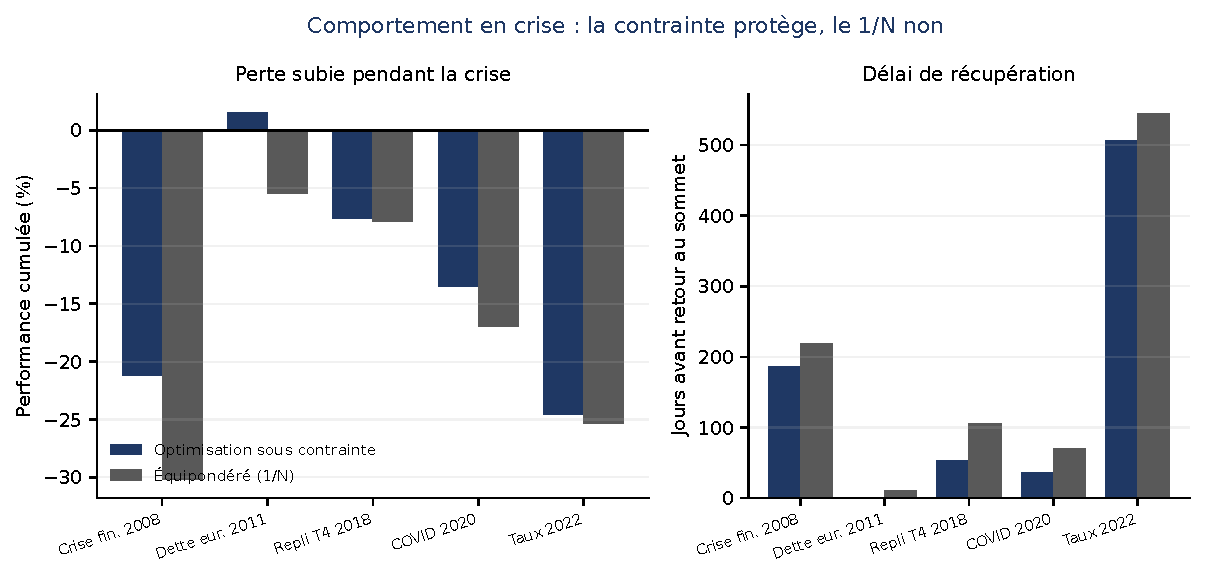
\includegraphics[width=\textwidth]{assets/figures/crises.pdf}
  \caption[Comportement en crise]{Comportement pendant les cinq crises retenues,
  sur l'univers ETF. À gauche, la performance cumulée sur la fenêtre~; à droite,
  le nombre de jours nécessaires pour retrouver le sommet précédent.}
  \label{fig:crises}
\end{figure}

Sur les cinq crises, \textbf{sans exception}, l'optimisation sous contrainte perd
moins, chute moins profondément et récupère plus vite que la diversification
naïve~:

\begin{itemize}
  \item lors de la crise financière de 2008, elle épargne \textbf{9,0 points} de
        performance et \textbf{9,3 points} de drawdown~;
  \item pendant la crise de la dette européenne, elle termine \textbf{positive}
        ($+1{,}6$~\%) là où l'équipondéré perd $5{,}4$~\%~;
  \item le \textbf{délai de récupération} est l'écart le plus régulier —
        37~jours contre 71 après le krach COVID, 53 contre 105 après le repli de
        2018, soit environ \textbf{deux fois moins de temps sous l'eau}.
\end{itemize}

\begin{remarquebox}
Le délai de récupération n'apparaît dans aucune des mesures classiques du
chapitre, alors qu'il est probablement le plus parlant pour un décideur~:
combien de temps le capital reste-t-il en dessous de sa valeur d'avant-crise ?
\end{remarquebox}

\paragraph{Attribution — ce que ce résultat ne dit pas.} Ce gain revient à la
\textbf{contrainte de portefeuille et au modèle de covariance} (P1 et P3), et non
spécifiquement à la couche de régime. Sur trois des cinq fenêtres, les trois
optimiseurs produisent des résultats identiques à la décimale près, pour deux
raisons mécaniques~: en régime baissier, le système à régime \emph{devient} la
variance minimale par construction~; et le plafond de 25~\% sur cinq actifs
contraint fortement l'allocation. L'attribuer au \emph{Machine Learning} serait
inexact.

% =============================================================================
\section{La détection de régime : une analyse exploratoire (P2)}
% =============================================================================

Le détecteur de régime est un modèle \textbf{non supervisé}~: aucune date de
crise, aucun label de récession ne lui a jamais été fourni. Il observe uniquement
le rendement du marché, sa volatilité et la corrélation moyenne entre actifs, et
classe chaque date de rééquilibrage en régime haussier ou baissier — \emph{en
temps réel}, à partir des seules données passées, sans savoir qu'une crise
commence.

\begin{figure}[htbp]
  \centering
  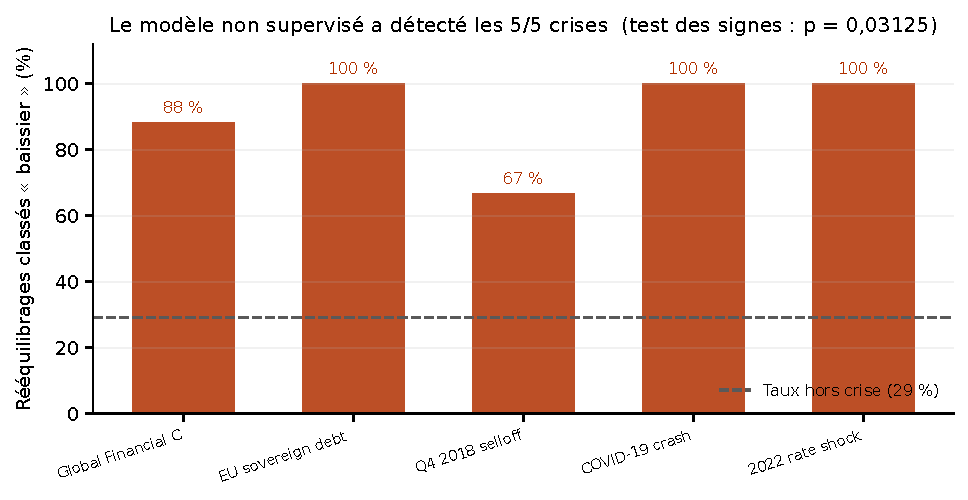
\includegraphics[width=0.94\textwidth]{assets/figures/detection_regime.pdf}
  \caption[Détection non supervisée des crises]{Proportion de rééquilibrages
  classés « baissier » pendant chacune des cinq crises, comparée au taux observé
  hors crise. Le modèle n'a reçu aucune information sur ces événements.}
  \label{fig:detection}
\end{figure}

Le résultat est net~: \textbf{91,7~\%} des rééquilibrages situés dans une fenêtre
de crise sont classés « baissier », contre \textbf{29,2~\%} en dehors — un
rapport de \textbf{3,13}, et les cinq crises dépassent le taux de base.

\begin{table}[htbp]
  \centering
\caption[Diagnostic de la détection]{Deux diagnostics encadrent le problème de
  dépendance sérielle. Ils sont rapportés pour transparence, non comme une
  confirmation statistique généralisable sur cinq événements.}
\label{tab:diagnostic_detection}
  \small
  \begin{tabular}{llp{7.4cm}}
    \toprule
    Diagnostic & Résultat & Lecture \\
    \midrule
    Test des signes \emph{(exploratoire)} & $p = 0{,}031$ &
      Chaque crise compte pour une observation ($n = 5$). Ce calcul évite la
      dépendance sérielle interne, mais cinq observations ne permettent pas une
      conclusion confirmatoire. \\
    Fisher exact \emph{(libéral)} & $p = 7{,}8 \times 10^{-13}$ &
      Traite 248 rééquilibrages mensuels corrélés comme indépendants~:
      optimiste. À ne jamais citer seul. \\
    \bottomrule
  \end{tabular}
\end{table}

\begin{resultatbox}{Association exploratoire, non preuve de détection}
Le détecteur est plus souvent dans l'état étiqueté « baissier » pendant les cinq
fenêtres étudiées. Le test des signes donne $p = 0{,}031$, mais cet indicateur
reste exploratoire~: l'échantillon contient cinq événements et « baissier » est
défini par le rendement moyen faible de l'état. Il ne doit pas être présenté comme
un résultat confirmatoire, ni comme une preuve de valeur économique.
\end{resultatbox}

\paragraph{La réserve qui doit accompagner ce résultat.} Le régime « baissier »
est \emph{défini} comme l'état de plus faible rendement moyen, et une crise est
par nature une période de faible rendement~: une part de l'association est donc
définitionnelle. Ce qui ne l'est pas, c'est que la détection soit \textbf{causale
et en temps réel}, et qu'elle ne se déclenche pas en permanence — le taux hors
crise reste à 29~\%, non à 80~\%. Le modèle ne crie pas au loup.

\begin{remarquebox}
Deux affirmations distinctes, à ne jamais confondre~: le détecteur produit une
lecture causale de l'état de marché, associée aux cinq fenêtres étudiées~; le fait
d'\textbf{agir} sur cette lecture n'a pas établi d'avantage économique robuste
face aux approches classiques.
\end{remarquebox}

% =============================================================================
\section{La contrainte fait plus que les modèles (P1)}
% =============================================================================

Le plafond de 25~\% par actif avait été retenu comme une contrainte de gestion
réaliste, non comme un outil de modélisation. En le faisant varier seul, tout le
reste étant fixé, on obtient le résultat le plus inattendu du projet.

\begin{figure}[htbp]
  \centering
  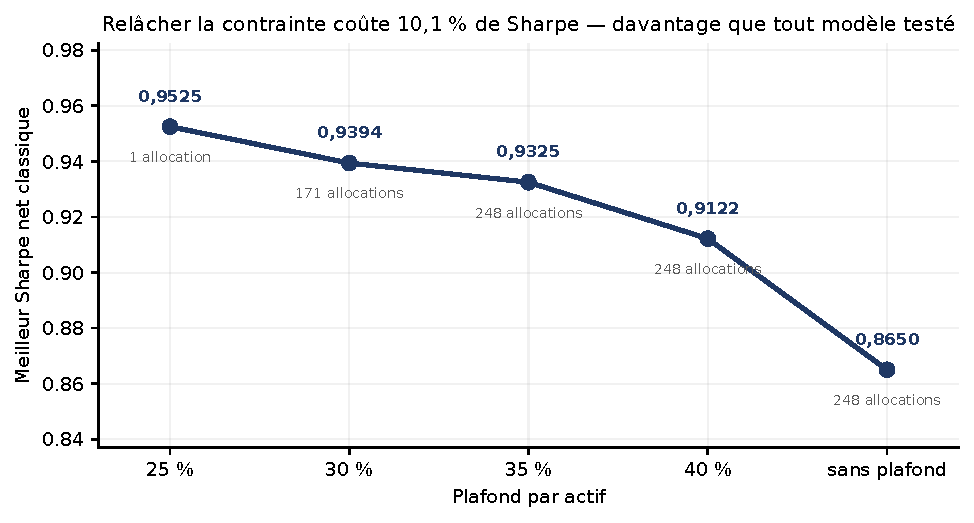
\includegraphics[width=0.94\textwidth]{assets/figures/plafond.pdf}
  \caption[Effet du plafond par actif]{Meilleur ratio de Sharpe classique en
  fonction du plafond par actif, sur 248~rééquilibrages et 20,7~ans. Le nombre
  d'allocations distinctes émises est indiqué sous chaque point.}
  \label{fig:plafond}
\end{figure}

Relâcher le plafond de 25~\% jusqu'à l'absence de contrainte fait chuter le
meilleur Sharpe classique de \textbf{0,9525 à 0,8650}, soit une perte de
\textbf{10,1~\%}, de façon monotone. C'est davantage que l'écart entre deux
modèles quelconques sur cet univers~: le rétrécissement de Ledoit-Wolf, l'EWMA,
le DCC-GARCH et la commutation de régime réunis déplacent moins le résultat.

Il s'agit du résultat de \textbf{Jagannathan et Ma (2003)} reproduit sur nos
données~: une contrainte de poids active équivaut mathématiquement à un
rétrécissement de la matrice de covariance. \textbf{La contrainte réalisait donc
déjà le contrôle d'erreur d'estimation (P1) que le \emph{Machine Learning} devait
apporter.}

Le nombre d'allocations distinctes éclaire le mécanisme~: à 25~\% sur cinq
actifs, $5 \times 0{,}25 = 1{,}25$, si bien que tout portefeuille admissible doit
placer au moins quatre actifs au plafond. La variance minimale n'émet alors
qu'\textbf{une seule} allocation sur 248~rééquilibrages~; à 30~\%, elle en émet
171. Sur cet univers, la contrainte — et non le modèle — détermine l'essentiel de
l'allocation.

\begin{remarquebox}
À présenter comme un résultat, non comme une limite~: le contrôle du risque le
plus efficace de ce système s'est révélé être la limite de position qu'un mandat
réel imposerait de toute façon. C'est précisément ce que le cadrage
« contraintes réalistes de gestion » du cahier des charges invitait à découvrir.
\end{remarquebox}

% =============================================================================
\section{Ce qui ne fonctionne pas : cinq pistes fermées}
% =============================================================================

La couche de prédiction de rendement — des modèles d'apprentissage supervisé
prédisant le rendement de chaque actif — n'a jamais dépassé la ligne de base.
Plutôt que de l'accepter, cinq explications possibles ont été testées
indépendamment, chacune avec un protocole pré-enregistré.

\begin{table}[htbp]
  \centering
  \caption[Les cinq pistes testées]{Cinq tentatives indépendantes de dépasser la
  ligne de base régime + covariance dynamique.}
  \label{tab:cinq-pistes}
  \small
  \begin{tabular}{p{7.4cm}p{7.2cm}}
    \toprule
    Piste testée & Verdict \\
    \midrule
    Prédiction de rendement calibrée honnêtement & indiscernable de la ligne de base \\
    5 fois plus d'historique de prix (univers marocain profond, 56\,000 lignes) &
      coefficient d'information $\times 2$ à $\times 4$, aucun avantage de portefeuille \\
    Données fondamentales point-in-time (P/E, P/B, P/S, D/E) &
      coefficient d'information $\times 2$, ratio de Sharpe en \textbf{baisse} \\
    Ré-sélection par pli, 74~\% de données hors échantillon en plus &
      intervalles $-28{,}6$~\%, classement instable \\
    Contrainte conditionnée au régime & réfutée par son propre contrôle \\
    \bottomrule
  \end{tabular}
\end{table}

Deux de ces études méritent d'être détaillées, car elles établissent un point de
méthode qui dépasse ce projet.

\paragraph{Précision de prédiction $\neq$ performance de portefeuille.} L'ajout
de données fondamentales a presque \emph{doublé} la capacité prédictive mesurée
du modèle (coefficient d'information de 0,028 à 0,058) — et a fait \emph{baisser}
le ratio de Sharpe du portefeuille correspondant. Le même phénomène est apparu
avec cinq fois plus d'historique de prix. Améliorer un modèle et améliorer un
portefeuille sont deux objectifs distincts~; le second ne découle pas
automatiquement du premier.

\paragraph{L'importance d'un contrôle destiné à réfuter.} L'étude sur la
contrainte conditionnée au régime incluait une variante \textbf{inversée},
délibérément construite dans la mauvaise direction. Sur le portefeuille EURAFRIC,
cette variante inversée est bien la pire — ce qui semblait confirmer l'existence
d'un effet de régime. Mais sur l'univers ETF, elle \emph{dépasse} la meilleure
variante « correcte ». Un effet qui change de signe selon l'univers n'est pas un
effet. Sans ce contrôle, la conclusion aurait été inverse.

\begin{resultatbox}{Ce que la convergence de ces cinq études démontre}
Le constat n'est pas que chaque idée a échoué individuellement, mais qu'à cette
taille d'échantillon, \textbf{l'évaluation ne peut pas résoudre des différences
de l'ordre de grandeur que ces idées produisent}. C'est l'affirmation
scientifique la plus défendable du projet, et elle n'est disponible que parce que
cinq tentatives indépendantes ont été menées avec un protocole identique.
\end{resultatbox}

% =============================================================================
\section{Le produit livré}
% =============================================================================

Le projet ne se limite pas à une étude~: il livre un outil utilisable, composé
d'une application web à deux pages et d'une interface REST, partageant une couche
de données unique — de sorte que deux surfaces ne puissent jamais afficher des
chiffres divergents pour la même stratégie.

\subsection{Page « Histoire de valeur » — destinée aux décideurs}

\begin{figure}[htbp]
  \centering
  \fbox{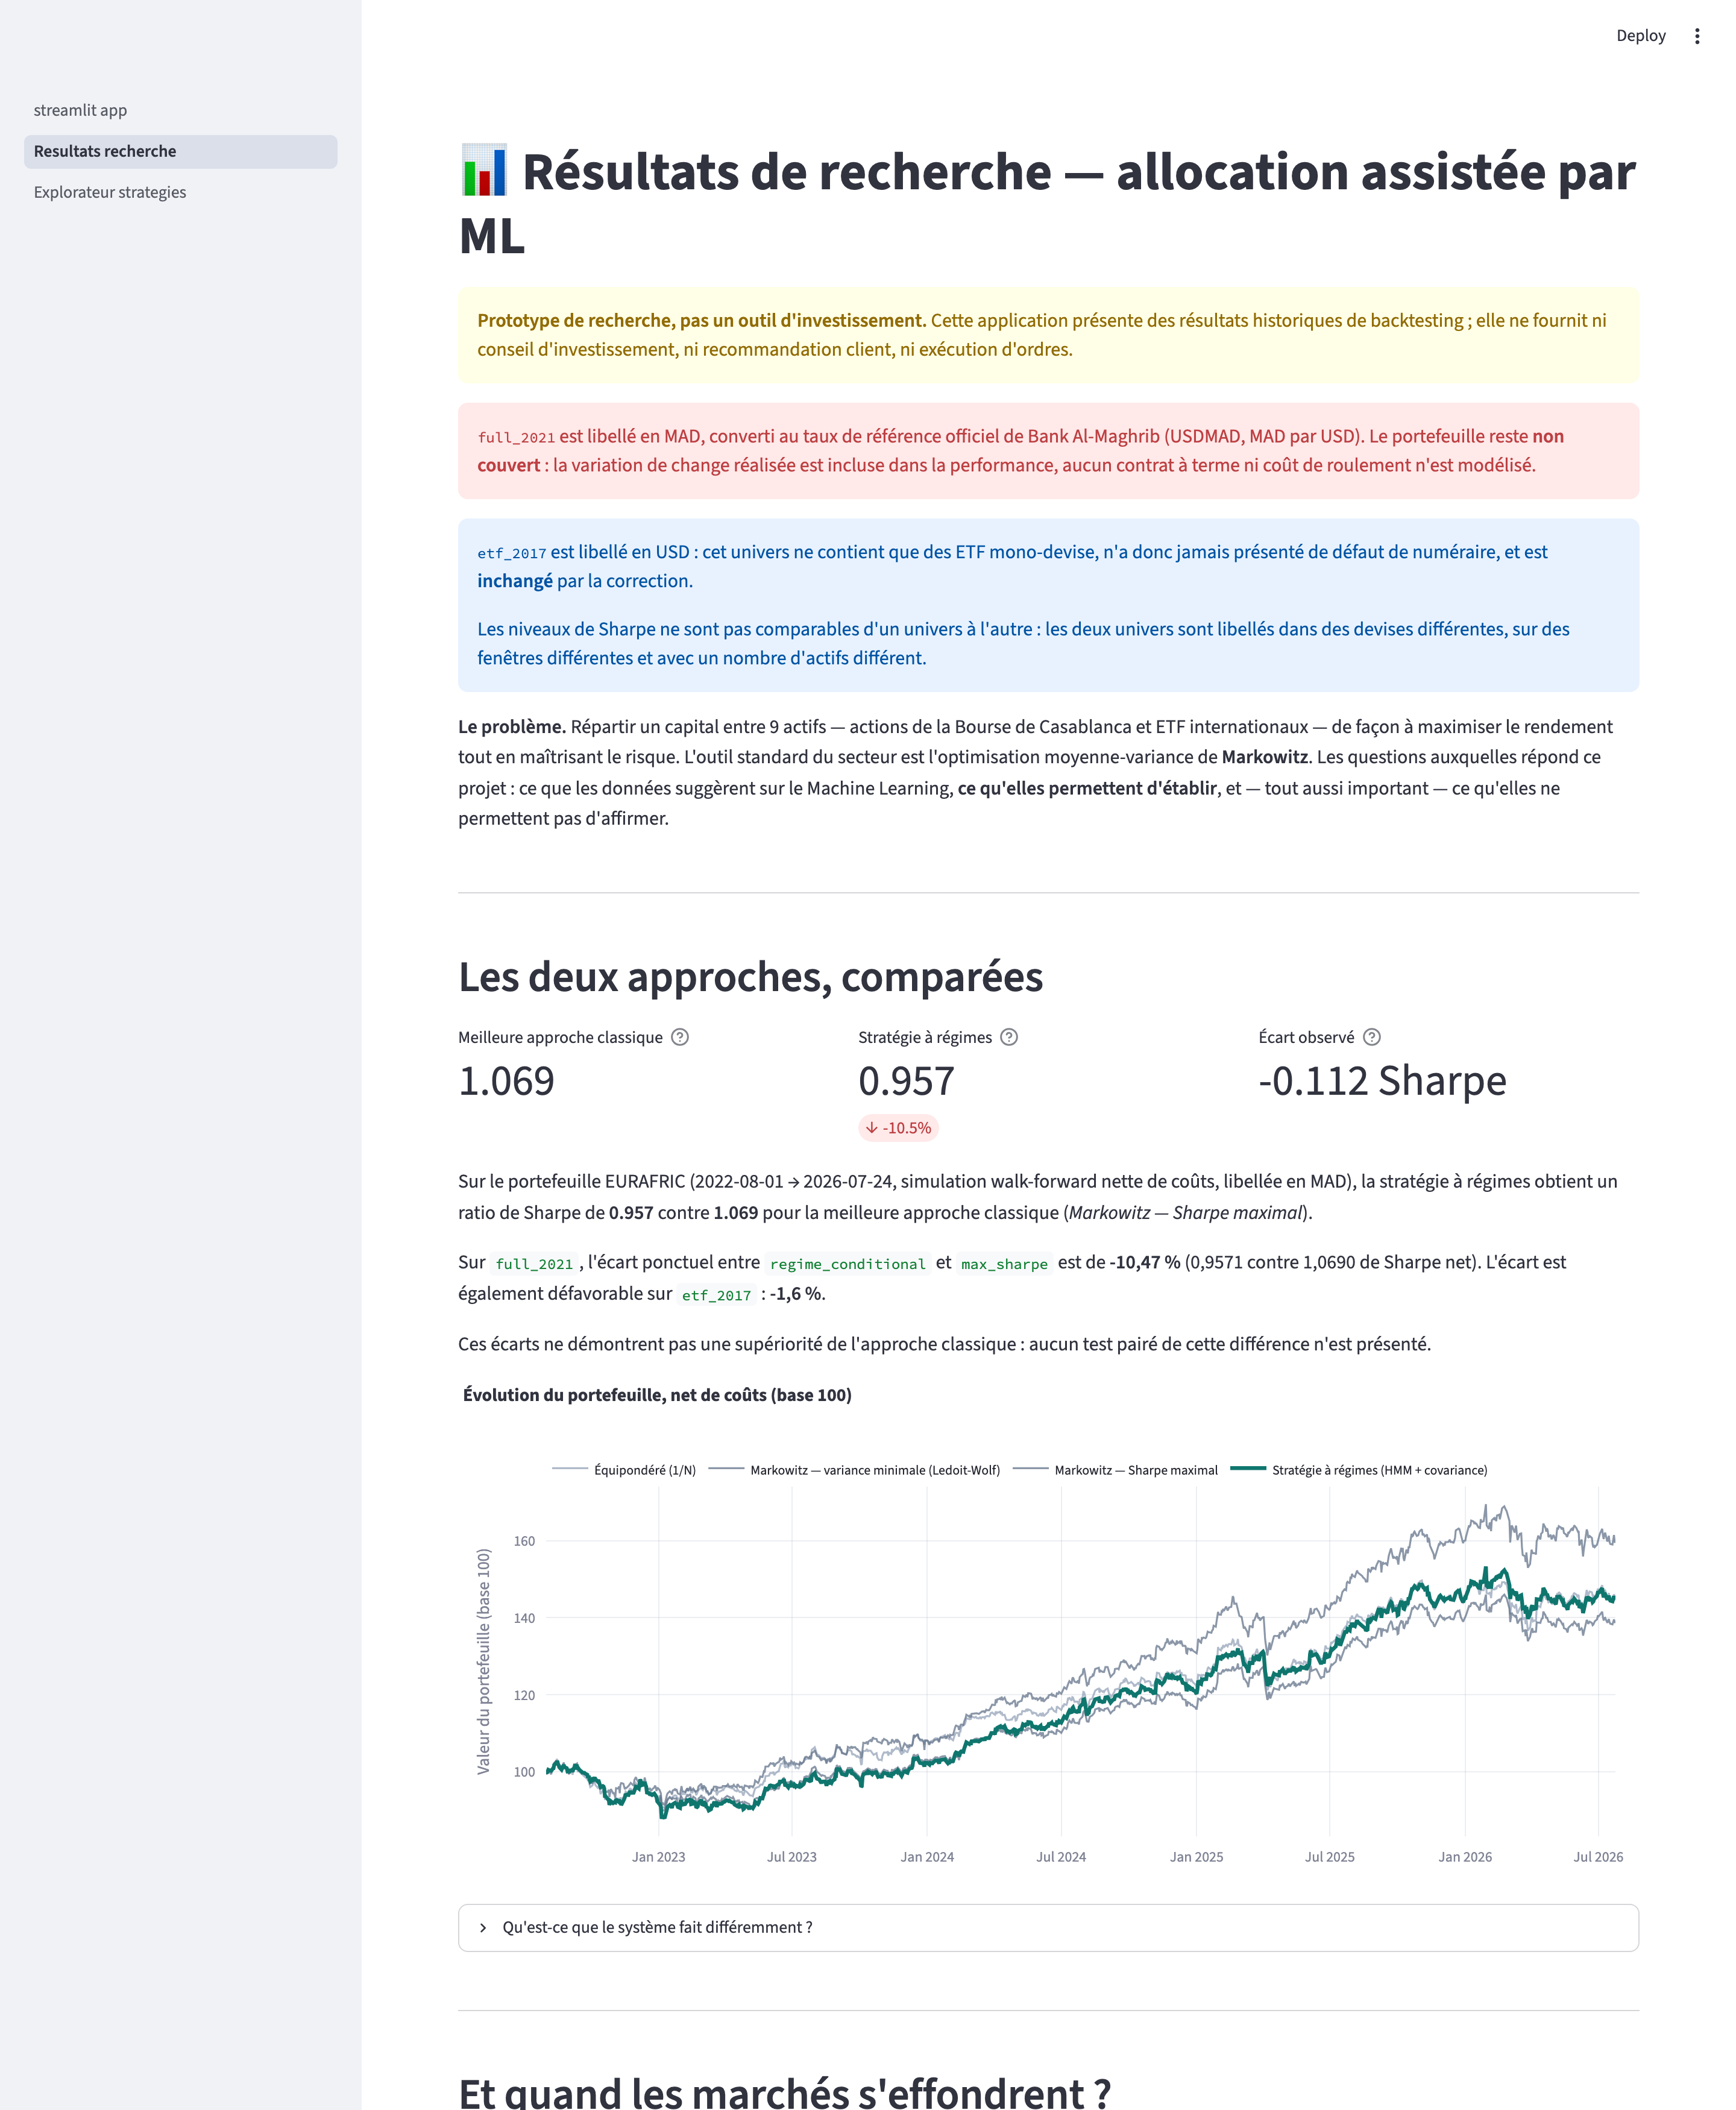
\includegraphics[width=0.93\textwidth]{assets/figures/dashboard_page1.png}}
  \caption[Tableau de bord — page décideur]{Page destinée aux décideurs. Elle
  présente d'abord le comportement en crise — le résultat le plus solide — puis
  seulement ensuite le ratio de Sharpe, dont l'écart n'est pas significatif.
  L'attribution honnête et les réserves statistiques sont affichées à l'écran, non
  reléguées en note.}
  \label{fig:dashboard1}
\end{figure}

Quatre contraintes d'intégrité sont imposées \emph{par le code} de cette page,
plutôt que laissées à la discipline de rédaction~:

\begin{enumerate}
  \item aucun chiffre n'est saisi en dur — tout est calculé à partir des
        artefacts versionnés, ce qu'un test vérifie en inspectant le code source~;
  \item chaque performance affichée est accompagnée de son intervalle de
        confiance, et le texte indique explicitement que les intervalles se
        chevauchent~;
  \item le cas défavorable — l'univers ETF, où le système perd — est affiché, non
        dissimulé~;
  \item la couche de prédiction de rendement n'est jamais présentée comme
        l'apport du projet, puisque cinq études ont établi qu'elle n'en apporte
        pas.
\end{enumerate}

\subsection{Page « Outil du gestionnaire » — destinée à l'usage métier}

\begin{figure}[htbp]
  \centering
  \fbox{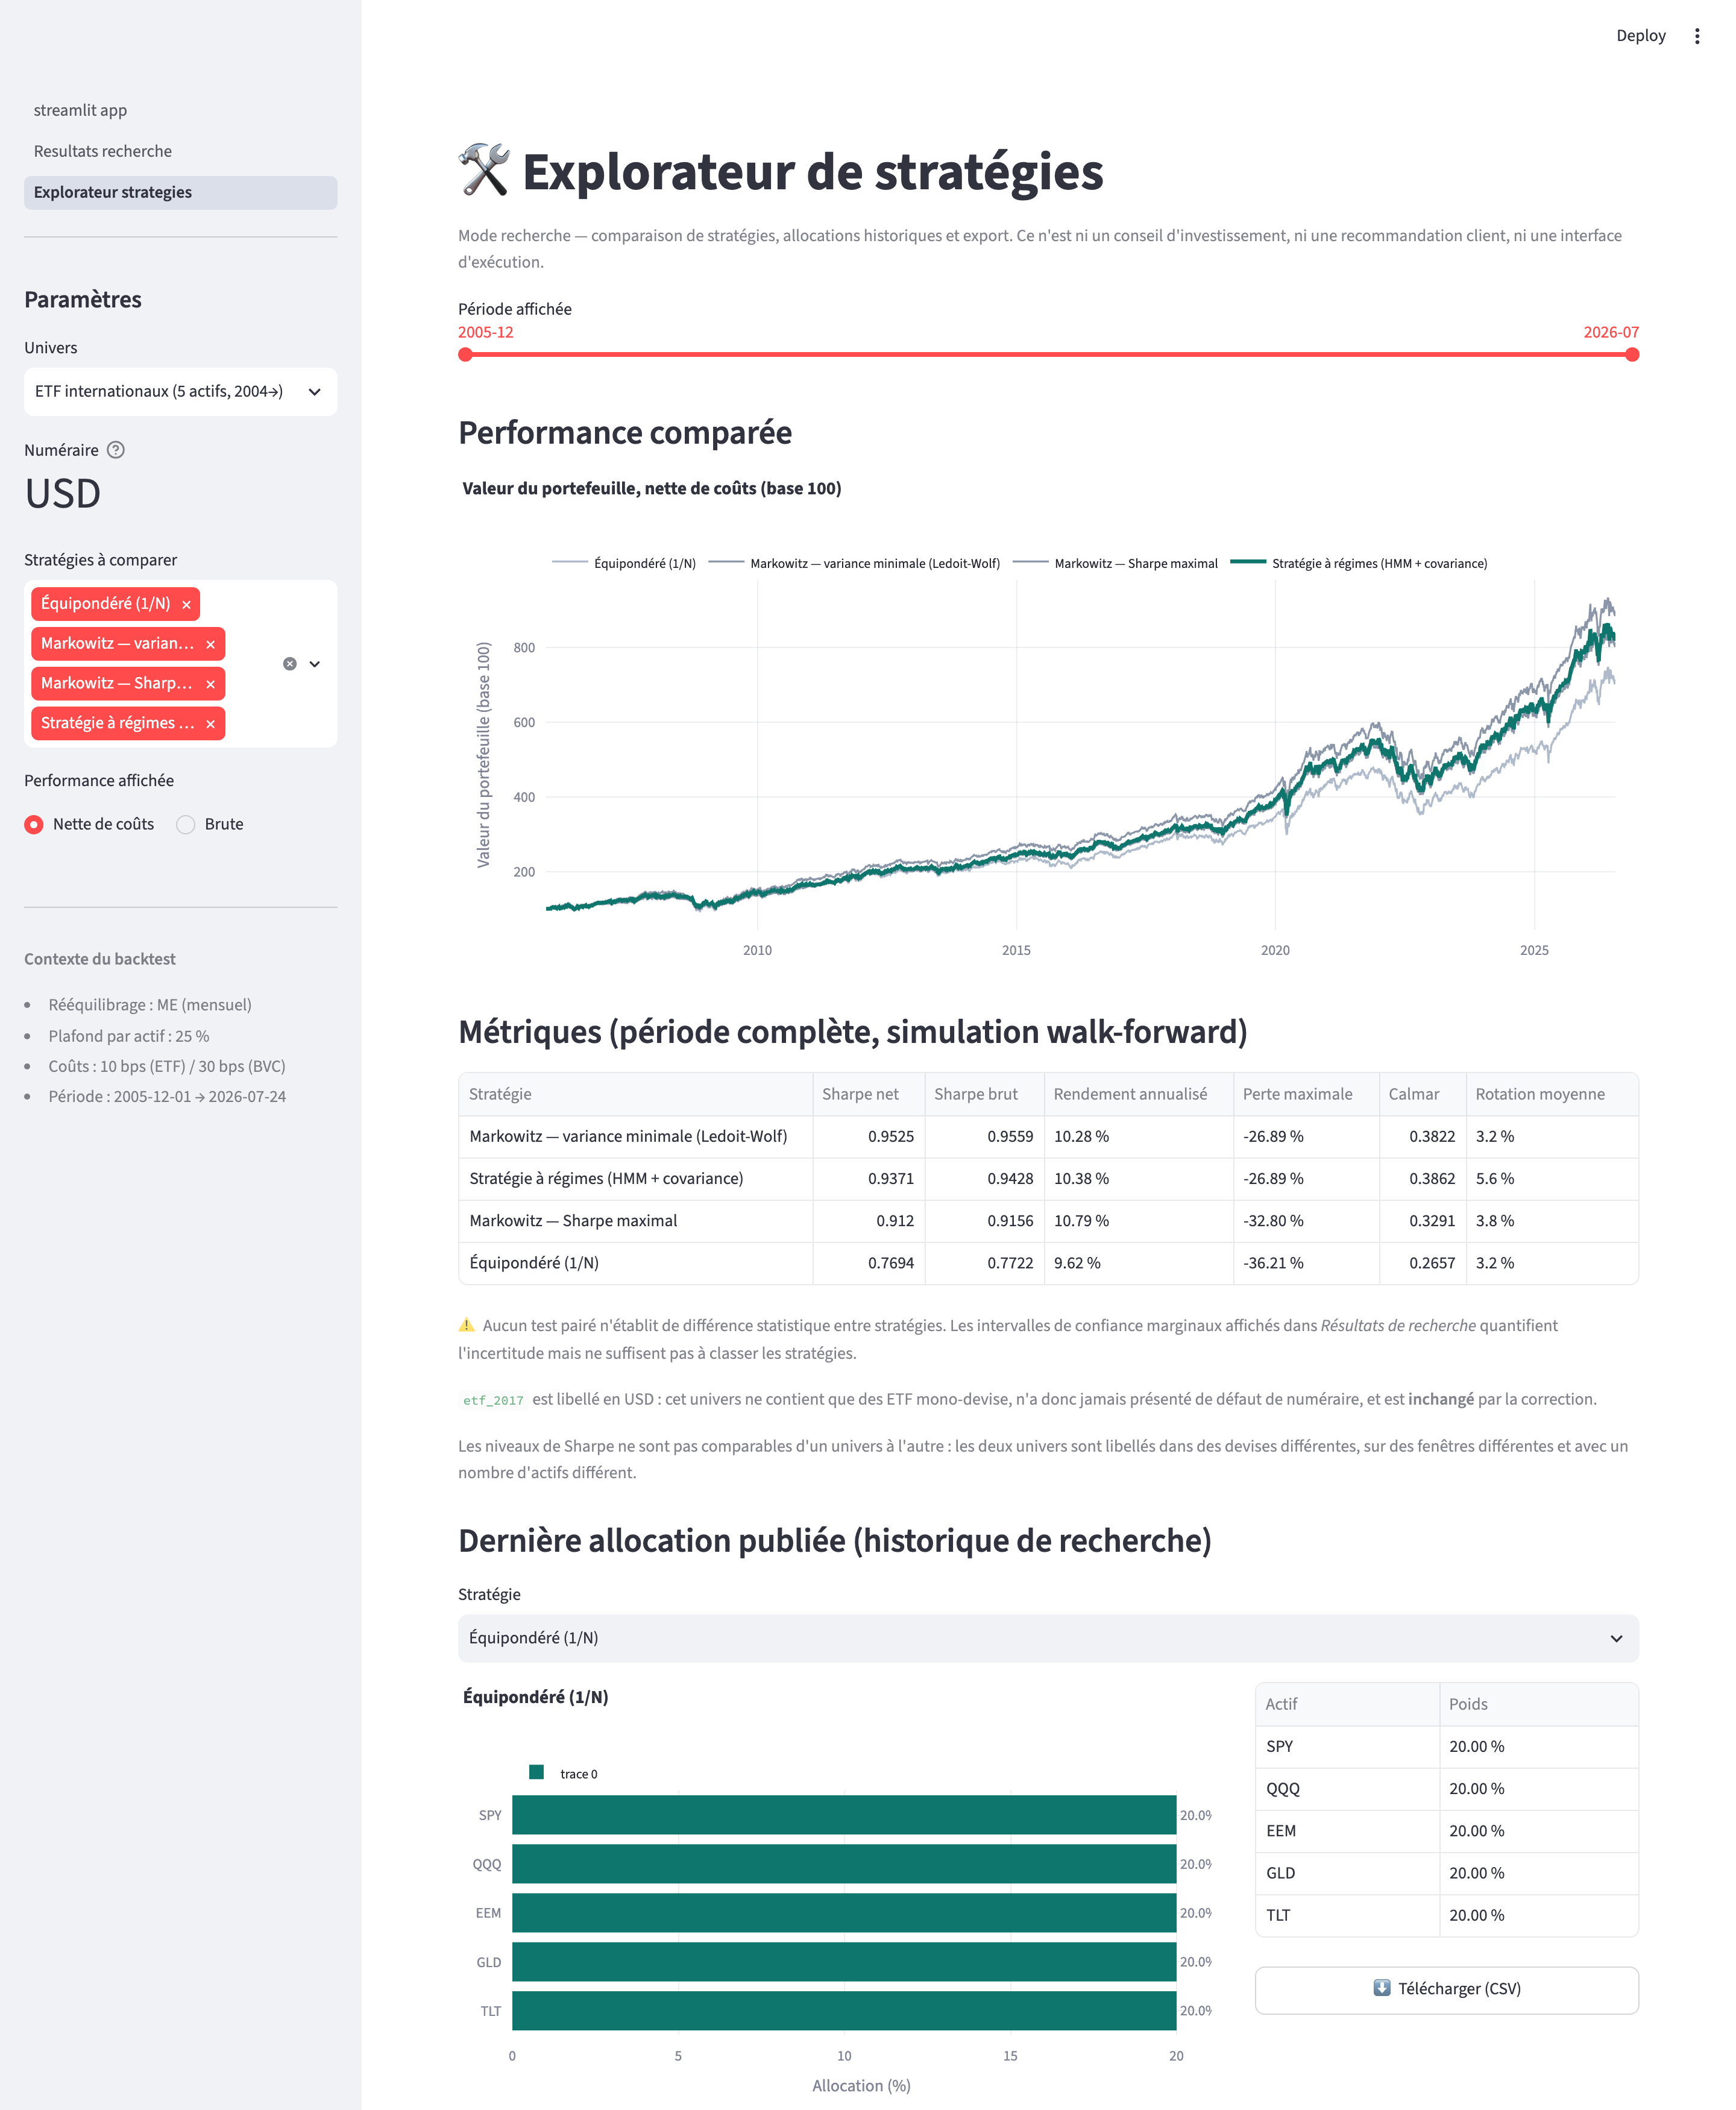
\includegraphics[width=0.93\textwidth]{assets/figures/dashboard_page2.png}}
  \caption[Tableau de bord — outil du gestionnaire]{Page métier~: comparaison de
  stratégies, métriques nettes de coûts, allocation cible et export CSV. Elle
  intègre également un explorateur de plafond, qui rend interactif le résultat de
  la section précédente.}
  \label{fig:dashboard2}
\end{figure}

Cette page ajoute un \textbf{explorateur de plafond}~: un curseur permettant de
faire varier la contrainte de position et d'observer immédiatement son effet sur
la performance. C'est le résultat le plus marquant du projet rendu manipulable
plutôt que consigné dans un tableau.

\subsection{L'interface REST}

Une API expose les mêmes artefacts pour un usage externe (\texttt{/strategies},
\texttt{/metrics}, \texttt{/equity}, \texttt{/weights}, \texttt{/compare},
\texttt{/crisis}). Elle est délibérément \emph{mince}~: elle sert des artefacts
versionnés et ne réentraîne jamais de modèle à la demande.

Deux points de conception méritent d'être signalés. D'une part, le point d'entrée
\texttt{/compare} renvoie toujours l'intervalle de confiance \emph{avec} l'écart
de performance~: un client ne peut pas récupérer le gain sans son incertitude.
D'autre part, \texttt{/crisis} expose l'analyse exploratoire avec sa réserve
d'attribution et ses limites d'inférence.

% =============================================================================
\section*{Synthèse du chapitre}
\addcontentsline{toc}{section}{Synthèse du chapitre}

\begin{itemize}
  \item \textbf{Exploré} — le détecteur de régime est plus souvent dans l'état
        « baissier » durant les cinq fenêtres étudiées. Le diagnostic $p = 0{,}031$
        est rapporté comme exploratoire, non confirmatoire.
  \item \textbf{Observé, non démontré} — le système à régimes dépasse le Markowitz
        classique de $6{,}2$~\% sur le portefeuille EURAFRIC et lui est inférieur
        de $1{,}6$~\% sur l'univers ETF. Le classement dépend du protocole
        d'évaluation et de la mesure retenue.
  \item \textbf{Testé, non établi} — sous validation strictement antérieure, les
        \textbf{huit} comparaisons pairées sur la fenêtre gelée ont un intervalle
        contenant zéro ($p$ de 0,066 à 0,939). Aucun modèle de signal n'établit de
        surperformance, ni contre la stratégie à régimes ni contre l'équipondéré,
        sur aucun des deux univers. C'est le résultat le mieux étayé du chapitre,
        parce que c'est le seul qui repose sur un test de la \emph{différence}
        plutôt que sur des intervalles marginaux.
  \item \textbf{Observé, robuste} — l'optimisation sous contrainte protège
        systématiquement mieux que la diversification naïve pendant les cinq
        crises, avec un délai de récupération environ deux fois plus court. Ce
        gain revient à la contrainte et à la covariance, non à la couche de
        régime.
  \item \textbf{Découvert} — le plafond de position, choisi comme règle métier,
        est le régulariseur le plus efficace du système~: 10,1~\% de Sharpe, plus
        que tout modèle testé.
  \item \textbf{Réfuté} — cinq pistes indépendantes visant à dépasser la ligne de
        base, dont deux établissant que précision de prédiction et performance de
        portefeuille sont des objectifs distincts.
\end{itemize}

Le chapitre suivant conclut en dressant le bilan de ce que le système apporte,
des limites qui subsistent, et des directions qu'un prolongement devrait
privilégier.
